\chapter{System Requirements, Architecture and Design}
\label{chap:architecture}

This chapter presents the comprehensive system requirements, architectural design, and development plan for the Pixelar platform.

\clearpage
\section{System Requirements}

\subsection{Functional Requirements}

The functional requirements define the specific behaviors and functions that the Pixelar system must provide.

\subsubsection{User Management Requirements}

\noindent
\begin{minipage}{\textwidth}
\centering
\captionof{table}{User Management Functional Requirements}
\label{tab:fr_user}
\small
\begin{tabular}{|l|p{7cm}|c|}
\hline
\textbf{ID} & \textbf{Requirement} & \textbf{Priority} \\
\hline
FR-U01 & Allow users to register using email and password & High \\
\hline
FR-U02 & Support Google OAuth authentication & High \\
\hline
FR-U03 & Maintain user sessions using JWT tokens & High \\
\hline
FR-U04 & Allow users to view and edit their profile & Medium \\
\hline
FR-U05 & Track user credit balance & High \\
\hline
FR-U06 & Support BYOK API key storage (client-side) & Medium \\
\hline
\end{tabular}
\end{minipage}
\vspace{0.5cm}

\subsubsection{Generation Requirements}

\noindent
\begin{minipage}{\textwidth}
\centering
\captionof{table}{Asset Generation Functional Requirements}
\label{tab:fr_gen}
\small
\begin{tabular}{|l|p{7cm}|c|}
\hline
\textbf{ID} & \textbf{Requirement} & \textbf{Priority} \\
\hline
FR-G01 & Generate sprite images from text prompts & High \\
\hline
FR-G02 & Support pixel art and 2D flat styles & High \\
\hline
FR-G03 & Support multiple viewpoints & High \\
\hline
FR-G04 & Allow color palette specification & Medium \\
\hline
FR-G05 & Generate scene/background images & High \\
\hline
FR-G06 & Generate animation frame sequences & High \\
\hline
FR-G07 & Maintain character consistency across frames & High \\
\hline
FR-G08 & Support 47 predefined animation actions & Medium \\
\hline
FR-G09 & Allow reference image upload & Medium \\
\hline
FR-G10 & Support multiple aspect ratios & Medium \\
\hline
\end{tabular}
\end{minipage}
\vspace{0.5cm}

\subsubsection{Project Management Requirements}

\noindent
\begin{minipage}{\textwidth}
\centering
\captionof{table}{Project Management Functional Requirements}
\label{tab:fr_project}
\small
\begin{tabular}{|l|p{7cm}|c|}
\hline
\textbf{ID} & \textbf{Requirement} & \textbf{Priority} \\
\hline
FR-P01 & Allow users to create projects & High \\
\hline
FR-P02 & Allow users to organize assets within projects & High \\
\hline
FR-P03 & Track generation history with metadata & Medium \\
\hline
FR-P04 & Allow project deletion (soft delete) & Medium \\
\hline
FR-P05 & Display recent sessions on dashboard & Low \\
\hline
\end{tabular}
\end{minipage}
\vspace{0.5cm}

\subsubsection{Export Requirements}

\noindent
\begin{minipage}{\textwidth}
\centering
\captionof{table}{Export Functional Requirements}
\label{tab:fr_export}
\small
\begin{tabular}{|l|p{7cm}|c|}
\hline
\textbf{ID} & \textbf{Requirement} & \textbf{Priority} \\
\hline
FR-E01 & Allow downloading individual generated images & High \\
\hline
FR-E02 & Generate sprite sheets from animation frames & High \\
\hline
FR-E03 & Convert sprite sheets to animated GIFs & Medium \\
\hline
FR-E04 & Support PNG format with transparency & High \\
\hline
\end{tabular}
\end{minipage}
\vspace{0.5cm}

\clearpage
\subsection{Non-Functional Requirements}

\subsubsection{Performance Requirements}

\noindent
\begin{minipage}{\textwidth}
\centering
\captionof{table}{Performance Non-Functional Requirements}
\label{tab:nfr_perf}
\small
\begin{tabular}{|l|p{6cm}|c|}
\hline
\textbf{ID} & \textbf{Requirement} & \textbf{Target} \\
\hline
NFR-P01 & Average sprite generation time & $<$ 15 seconds \\
\hline
NFR-P02 & API response time (non-generation) & $<$ 500 ms \\
\hline
NFR-P03 & Page load time & $<$ 3 seconds \\
\hline
NFR-P04 & Concurrent user support & $>$ 100 users \\
\hline
NFR-P05 & Image upload time & $<$ 2 seconds \\
\hline
\end{tabular}
\end{minipage}
\vspace{0.5cm}

\subsubsection{Reliability Requirements}

\noindent
\begin{minipage}{\textwidth}
\centering
\captionof{table}{Reliability Non-Functional Requirements}
\label{tab:nfr_rel}
\small
\begin{tabular}{|l|p{6cm}|c|}
\hline
\textbf{ID} & \textbf{Requirement} & \textbf{Target} \\
\hline
NFR-R01 & System uptime & $>$ 99.5\% \\
\hline
NFR-R02 & Generation success rate & $>$ 95\% \\
\hline
NFR-R03 & Data backup frequency & Daily \\
\hline
NFR-R04 & Mean time to recovery & $<$ 1 hour \\
\hline
\end{tabular}
\end{minipage}
\vspace{0.5cm}

\subsubsection{Security Requirements}

\noindent
\begin{minipage}{\textwidth}
\centering
\captionof{table}{Security Non-Functional Requirements}
\label{tab:nfr_sec}
\small
\begin{tabular}{|l|p{9cm}|}
\hline
\textbf{ID} & \textbf{Requirement} \\
\hline
NFR-S01 & All API endpoints require authentication except public routes \\
\hline
NFR-S02 & User passwords hashed using industry-standard algorithms \\
\hline
NFR-S03 & BYOK API keys stored client-side only, never on server \\
\hline
NFR-S04 & All data transmission uses HTTPS encryption \\
\hline
NFR-S05 & JWT tokens expire after 1 hour \\
\hline
\end{tabular}
\end{minipage}
\vspace{0.5cm}

\subsubsection{Usability Requirements}

\noindent
\begin{minipage}{\textwidth}
\centering
\captionof{table}{Usability Non-Functional Requirements}
\label{tab:nfr_use}
\small
\begin{tabular}{|l|p{9cm}|}
\hline
\textbf{ID} & \textbf{Requirement} \\
\hline
NFR-U01 & Interface responsive across desktop and tablet devices \\
\hline
NFR-U02 & Users generate first asset within 5 minutes of registration \\
\hline
NFR-U03 & Error messages are clear and actionable \\
\hline
NFR-U04 & Visual feedback provided during generation processes \\
\hline
\end{tabular}
\end{minipage}
\vspace{0.5cm}

\clearpage
\section{System Flow Chart}

The following flow chart illustrates the primary user workflow for generating game assets.

\noindent
\begin{minipage}{\textwidth}
\centering
\begin{tikzpicture}[
    node distance=1.2cm,
    startstop/.style={rectangle, rounded corners, minimum width=2.5cm, minimum height=0.8cm, text centered, draw=black, fill=red!30, font=\small},
    process/.style={rectangle, minimum width=2.5cm, minimum height=0.8cm, text centered, draw=black, fill=blue!20, font=\small},
    decision/.style={diamond, minimum width=2cm, minimum height=0.8cm, text centered, draw=black, fill=green!20, aspect=2, font=\small},
    io/.style={trapezium, trapezium left angle=70, trapezium right angle=110, minimum width=2.5cm, minimum height=0.8cm, text centered, draw=black, fill=orange!20, font=\small},
    arrow/.style={thick,->,>=stealth}
]

\node (start) [startstop] {Start};
\node (login) [decision, below of=start, yshift=-0.3cm] {Logged In?};
\node (auth) [process, right of=login, xshift=2.5cm] {Authenticate};
\node (select) [process, below of=login, yshift=-0.3cm] {Select Asset Type};
\node (config) [io, below of=select] {Configure Params};
\node (haskey) [decision, below of=config, yshift=-0.3cm] {Has BYOK?};
\node (usebyok) [process, right of=haskey, xshift=2.5cm] {Use User Key};
\node (useplatform) [process, left of=haskey, xshift=-2.5cm] {Use Platform Key};
\node (generate) [process, below of=haskey, yshift=-0.3cm] {Generate Asset};
\node (success) [decision, below of=generate, yshift=-0.3cm] {Success?};
\node (retry) [process, right of=success, xshift=2.5cm] {Retry/Modify};
\node (save) [process, below of=success, yshift=-0.3cm] {Save to Project};
\node (download) [io, below of=save] {Download Asset};
\node (end) [startstop, below of=download] {End};

\draw [arrow] (start) -- (login);
\draw [arrow] (login) -- node[anchor=south] {No} (auth);
\draw [arrow] (auth) |- (select);
\draw [arrow] (login) -- node[anchor=east] {Yes} (select);
\draw [arrow] (select) -- (config);
\draw [arrow] (config) -- (haskey);
\draw [arrow] (haskey) -- node[anchor=south] {Yes} (usebyok);
\draw [arrow] (haskey) -- node[anchor=south] {No} (useplatform);
\draw [arrow] (usebyok) |- (generate);
\draw [arrow] (useplatform) |- (generate);
\draw [arrow] (generate) -- (success);
\draw [arrow] (success) -- node[anchor=south] {No} (retry);
\draw [arrow] (retry) |- (config);
\draw [arrow] (success) -- node[anchor=east] {Yes} (save);
\draw [arrow] (save) -- (download);
\draw [arrow] (download) -- (end);

\end{tikzpicture}
\captionof{figure}{Asset Generation Flow Chart}
\label{fig:flowchart}
\end{minipage}
\vspace{0.5cm}

\subsection{Detailed Process Flows}

\textbf{Sprite Generation Flow:}
\begin{enumerate}
    \item User navigates to Sprite Generator page
    \item User selects sprite type (Character/Object)
    \item User enters text prompt describing desired sprite
    \item User configures parameters (style, viewpoint, aspect ratio, colors)
    \item System validates user credits or BYOK key
    \item System constructs optimized prompt and calls AI API
    \item System uploads images to blob storage and saves metadata
    \item User previews, downloads, or saves to project
\end{enumerate}

\textbf{Animation Generation Flow:}
\begin{enumerate}
    \item User uploads character image
    \item User selects animation action from library (47 actions)
    \item User configures view type and direction
    \item System generates each frame with character reference
    \item System assembles frames into animation preview
    \item User exports as sprite sheet or GIF
\end{enumerate}

\clearpage
\section{Use Case Diagram}

\noindent
\begin{minipage}{\textwidth}
\centering
\begin{tikzpicture}[
    actor/.style={circle, draw, minimum size=0.8cm, font=\small},
    usecase/.style={ellipse, draw, minimum width=2cm, minimum height=0.8cm, text centered, text width=2cm, font=\small},
    system/.style={rectangle, draw, dashed, minimum width=9cm, minimum height=10cm}
]

\node[system, label=above:{\textbf{Pixelar System}}] (system) at (4.5,0) {};

\node[actor, label=below:{Guest}] (guest) at (-1, 2) {};
\node[actor, label=below:{User}] (user) at (-1, -2) {};
\node[actor, label=below:{AI Provider}] (ai) at (10, 0) {};

\node[usecase] (register) at (2.5, 3.5) {Register};
\node[usecase] (login) at (2.5, 2) {Login};
\node[usecase] (viewhome) at (2.5, 0.5) {View Home};
\node[usecase] (gensprite) at (4.5, -1) {Gen Sprite};
\node[usecase] (genscene) at (4.5, -2.5) {Gen Scene};
\node[usecase] (genanim) at (4.5, -4) {Gen Animation};
\node[usecase] (manageproj) at (6.5, 1) {Manage Projects};
\node[usecase] (download) at (6.5, -1) {Download};
\node[usecase] (managebyok) at (6.5, -2.5) {Manage BYOK};
\node[usecase] (processgen) at (8, -1) {Process};

\draw (guest) -- (register);
\draw (guest) -- (login);
\draw (guest) -- (viewhome);
\draw (user) -- (login);
\draw (user) -- (gensprite);
\draw (user) -- (genscene);
\draw (user) -- (genanim);
\draw (user) -- (manageproj);
\draw (user) -- (download);
\draw (user) -- (managebyok);
\draw (ai) -- (processgen);

\draw[dashed, ->] (gensprite) -- (processgen);
\draw[dashed, ->] (genscene) -- (processgen);
\draw[dashed, ->] (genanim) -- (processgen);

\end{tikzpicture}
\captionof{figure}{Use Case Diagram}
\label{fig:usecase}
\end{minipage}
\vspace{0.5cm}

\clearpage
\subsection{Use Case Descriptions}

\noindent
\begin{minipage}{\textwidth}
\centering
\captionof{table}{Use Case: Generate Sprite (UC-01)}
\label{tab:uc_sprite}
\small
\begin{tabular}{|p{3cm}|p{9cm}|}
\hline
\textbf{Use Case ID} & UC-01 \\
\hline
\textbf{Name} & Generate Sprite \\
\hline
\textbf{Actor} & Authenticated User \\
\hline
\textbf{Description} & User generates sprite images using AI based on text prompts \\
\hline
\textbf{Preconditions} & User logged in; has credits or BYOK key \\
\hline
\textbf{Postconditions} & Sprites saved; credits deducted (if applicable) \\
\hline
\textbf{Main Flow} & 
1. Navigate to Sprite Generator \newline
2. Enter prompt and configure parameters \newline
3. Click Generate \newline
4. System validates and calls AI \newline
5. System displays generated sprites \newline
6. User downloads or saves to project \\
\hline
\textbf{Alternative Flow} & 
A1. Insufficient credits: Show error \newline
A2. Generation fails: Allow retry \\
\hline
\end{tabular}
\end{minipage}
\vspace{0.5cm}

\noindent
\begin{minipage}{\textwidth}
\centering
\captionof{table}{Use Case: Generate Animation (UC-02)}
\label{tab:uc_anim}
\small
\begin{tabular}{|p{3cm}|p{9cm}|}
\hline
\textbf{Use Case ID} & UC-02 \\
\hline
\textbf{Name} & Generate Animation \\
\hline
\textbf{Actor} & Authenticated User \\
\hline
\textbf{Description} & User generates animation frame sequences from character image \\
\hline
\textbf{Preconditions} & User logged in; has character image; has credits/BYOK \\
\hline
\textbf{Postconditions} & Animation frames saved; sprite sheet available \\
\hline
\textbf{Main Flow} & 
1. Upload character image \newline
2. Select animation action \newline
3. Configure view and direction \newline
4. System generates frames sequentially \newline
5. System displays animation preview \newline
6. User exports sprite sheet or GIF \\
\hline
\end{tabular}
\end{minipage}
\vspace{0.5cm}

\noindent
\begin{minipage}{\textwidth}
\centering
\captionof{table}{Use Case: Manage Projects (UC-03)}
\label{tab:uc_project}
\small
\begin{tabular}{|p{3cm}|p{9cm}|}
\hline
\textbf{Use Case ID} & UC-03 \\
\hline
\textbf{Name} & Manage Projects \\
\hline
\textbf{Actor} & Authenticated User \\
\hline
\textbf{Description} & User creates, views, updates, and deletes projects \\
\hline
\textbf{Preconditions} & User is logged in \\
\hline
\textbf{Postconditions} & Project changes persisted to database \\
\hline
\textbf{Main Flow} & 
1. Navigate to Projects page \newline
2. View list of existing projects \newline
3. Create new or select existing project \newline
4. View project details and assets \newline
5. Update or delete project \\
\hline
\end{tabular}
\end{minipage}
\vspace{0.5cm}

\clearpage
\section{Software Development Plan}

\subsection{The Software Architecture}

The Pixelar platform follows a modern three-tier architecture with clear separation of concerns.

\subsubsection{High-Level Architecture}

\noindent
\begin{minipage}{\textwidth}
\centering
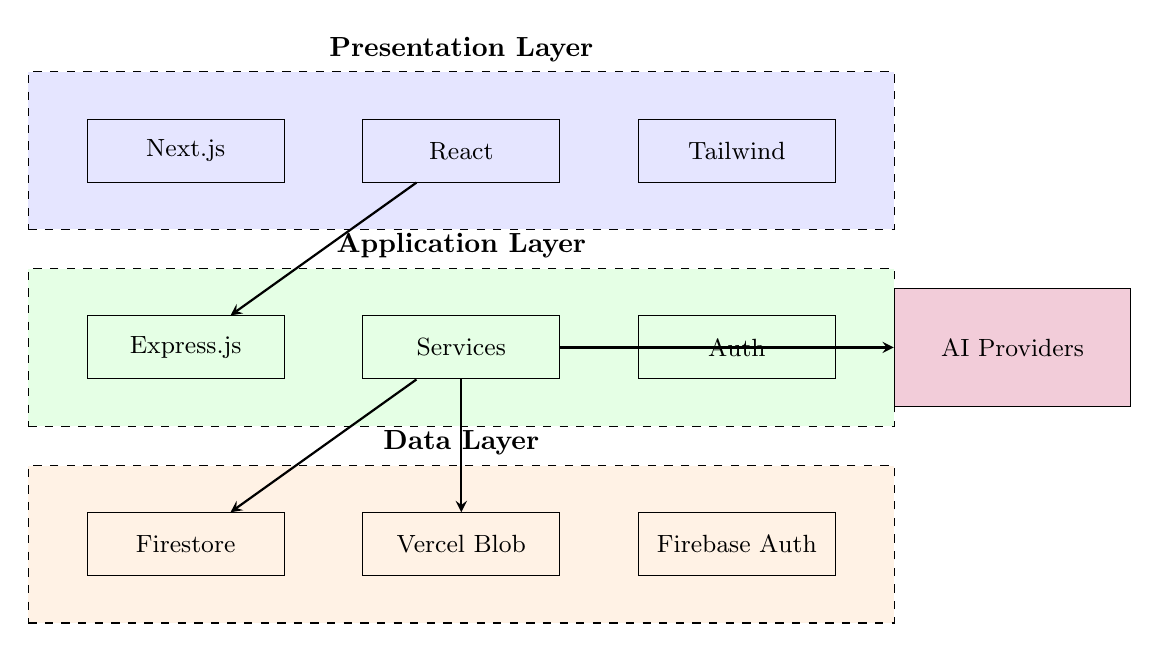
\begin{tikzpicture}[
    box/.style={rectangle, draw, minimum width=2.5cm, minimum height=0.8cm, text centered, font=\small},
    bigbox/.style={rectangle, draw, minimum width=3cm, minimum height=1.5cm, text centered, font=\small},
    layer/.style={rectangle, draw, dashed, minimum width=11cm, minimum height=2cm},
    arrow/.style={thick, ->, >=stealth}
]

\node[layer, fill=blue!10, label=above:{\textbf{Presentation Layer}}] (pres) at (0, 5) {};
\node[layer, fill=green!10, label=above:{\textbf{Application Layer}}] (app) at (0, 2.5) {};
\node[layer, fill=orange!10, label=above:{\textbf{Data Layer}}] (data) at (0, 0) {};

\node[box] (nextjs) at (-3.5, 5) {Next.js};
\node[box] (react) at (0, 5) {React};
\node[box] (tailwind) at (3.5, 5) {Tailwind};

\node[box] (express) at (-3.5, 2.5) {Express.js};
\node[box] (services) at (0, 2.5) {Services};
\node[box] (auth) at (3.5, 2.5) {Auth};

\node[box] (firestore) at (-3.5, 0) {Firestore};
\node[box] (blob) at (0, 0) {Vercel Blob};
\node[box] (firebase) at (3.5, 0) {Firebase Auth};

\node[bigbox, fill=purple!20] (ai) at (7, 2.5) {AI Providers};

\draw[arrow] (react) -- (express);
\draw[arrow] (services) -- (firestore);
\draw[arrow] (services) -- (blob);
\draw[arrow] (services) -- (ai);

\end{tikzpicture}
\captionof{figure}{High-Level System Architecture}
\label{fig:architecture}
\end{minipage}
\vspace{0.5cm}

\subsubsection{Frontend Architecture}

The frontend follows a component-based architecture using React and Next.js:

\begin{lstlisting}[language=bash, caption={Frontend Directory Structure}]
frontend/
├── app/           # Next.js App Router pages
├── components/    # Reusable UI components
├── contexts/      # React context providers
├── hooks/         # Custom React hooks
├── lib/           # Utility functions
└── public/        # Static assets
\end{lstlisting}

\subsubsection{Backend Architecture}

The backend implements a service-oriented architecture:

\begin{lstlisting}[language=bash, caption={Backend Directory Structure}]
Backend/
├── api/
│   ├── index.ts       # Express entry point
│   └── routes/        # API route handlers
├── services/          # Business logic
├── lib/               # Shared utilities
├── types/             # TypeScript definitions
└── tests/             # Test suite
\end{lstlisting}

\clearpage
\subsubsection{Database Schema Design}

\noindent
\begin{minipage}{\textwidth}
\centering
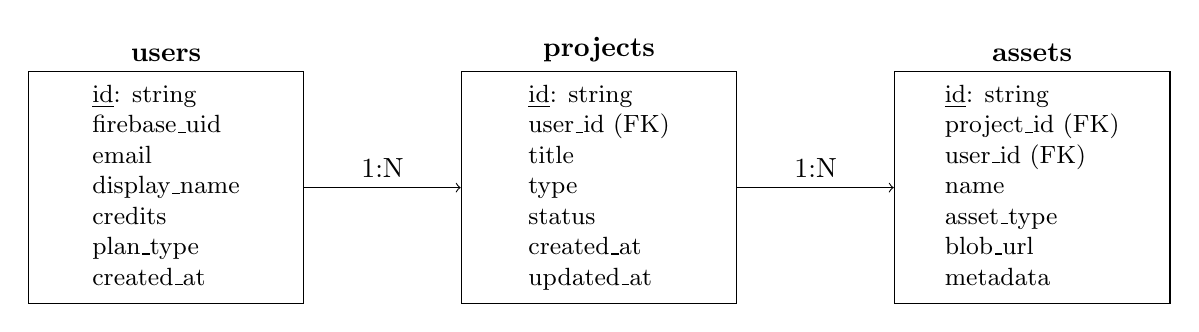
\begin{tikzpicture}[
    entity/.style={rectangle, draw, minimum width=3.5cm, minimum height=2.5cm, text centered, font=\small}
]

\node[entity, label=above:{\textbf{users}}] (users) at (0, 0) {
    \begin{tabular}{l}
    \underline{id}: string \\
    firebase\_uid \\
    email \\
    display\_name \\
    credits \\
    plan\_type \\
    created\_at
    \end{tabular}
};

\node[entity, label=above:{\textbf{projects}}] (projects) at (5.5, 0) {
    \begin{tabular}{l}
    \underline{id}: string \\
    user\_id (FK) \\
    title \\
    type \\
    status \\
    created\_at \\
    updated\_at
    \end{tabular}
};

\node[entity, label=above:{\textbf{assets}}] (assets) at (11, 0) {
    \begin{tabular}{l}
    \underline{id}: string \\
    project\_id (FK) \\
    user\_id (FK) \\
    name \\
    asset\_type \\
    blob\_url \\
    metadata
    \end{tabular}
};

\draw[->] (users.east) -- node[above] {1:N} (projects.west);
\draw[->] (projects.east) -- node[above] {1:N} (assets.west);

\end{tikzpicture}
\captionof{figure}{Database Entity Relationship Diagram}
\label{fig:erd}
\end{minipage}
\vspace{0.5cm}

\subsubsection{API Architecture}

\noindent
\begin{minipage}{\textwidth}
\centering
\captionof{table}{API Endpoint Architecture}
\label{tab:api_arch}
\small
\begin{tabular}{|l|l|l|p{4.5cm}|}
\hline
\textbf{Method} & \textbf{Endpoint} & \textbf{Auth} & \textbf{Description} \\
\hline
\multicolumn{4}{|c|}{\textbf{Generation Endpoints}} \\
\hline
POST & /api/generate/sprite & Yes & Generate sprite images \\
\hline
POST & /api/generate/scene & Yes & Generate scene images \\
\hline
POST & /api/generate/animation & Yes & Generate animation frames \\
\hline
GET & /api/generate/history & Yes & Get generation history \\
\hline
\multicolumn{4}{|c|}{\textbf{User Endpoints}} \\
\hline
GET & /api/user/profile & Yes & Get user profile \\
\hline
PUT & /api/user/profile & Yes & Update user profile \\
\hline
POST & /api/user/credits/deduct & Yes & Deduct credits \\
\hline
\multicolumn{4}{|c|}{\textbf{Project Endpoints}} \\
\hline
GET & /api/projects & Yes & List user projects \\
\hline
POST & /api/projects & Yes & Create project \\
\hline
GET & /api/projects/:id & Yes & Get project details \\
\hline
PUT & /api/projects/:id & Yes & Update project \\
\hline
DELETE & /api/projects/:id & Yes & Delete project \\
\hline
\end{tabular}
\end{minipage}
\vspace{0.5cm}

\clearpage
\subsection{Number of Development Iterations}

The project was developed using Agile Scrum methodology in four two-week iterations.

\noindent
\begin{minipage}{\textwidth}
\centering
\captionof{table}{Development Iteration Summary}
\label{tab:iterations}
\small
\begin{tabular}{|c|l|c|c|l|}
\hline
\textbf{Iter.} & \textbf{Focus Area} & \textbf{Duration} & \textbf{Semester} & \textbf{Status} \\
\hline
1 & Core Infrastructure & 2 weeks & 7 & Completed \\
\hline
2 & AI Generation Service & 2 weeks & 7 & Completed \\
\hline
3 & Animation System & 2 weeks & 8 & Completed \\
\hline
4 & Project Management & 2 weeks & 8 & Completed \\
\hline
\end{tabular}
\end{minipage}
\vspace{0.5cm}

\subsubsection{Iteration 1: Core Infrastructure (Semester 7)}

\textbf{Duration}: Weeks 1-2

\textbf{Objectives}: Establish project structure, implement authentication, design database schema, create frontend shell.

\noindent
\begin{minipage}{\textwidth}
\centering
\captionof{table}{Iteration 1 Sprint Backlog}
\label{tab:sprint1}
\small
\begin{tabular}{|p{6cm}|c|c|}
\hline
\textbf{Task} & \textbf{Points} & \textbf{Status} \\
\hline
Set up Next.js project structure & 3 & Done \\
\hline
Set up Express.js backend & 3 & Done \\
\hline
Implement Firebase Auth integration & 5 & Done \\
\hline
Create authentication middleware & 3 & Done \\
\hline
Design Firestore schema & 5 & Done \\
\hline
Implement User Service & 5 & Done \\
\hline
Create login/register pages & 5 & Done \\
\hline
Implement profile management & 3 & Done \\
\hline
Set up Vercel deployment & 2 & Done \\
\hline
Write unit tests & 5 & Done \\
\hline
\textbf{Total} & \textbf{39} & \\
\hline
\end{tabular}
\end{minipage}
\vspace{0.5cm}

\subsubsection{Iteration 2: AI Generation Service (Semester 7)}

\textbf{Duration}: Weeks 3-4

\textbf{Objectives}: Integrate AI providers, implement prompt engineering, create generation endpoints, implement BYOK.

\noindent
\begin{minipage}{\textwidth}
\centering
\captionof{table}{Iteration 2 Sprint Backlog}
\label{tab:sprint2}
\small
\begin{tabular}{|p{6cm}|c|c|}
\hline
\textbf{Task} & \textbf{Points} & \textbf{Status} \\
\hline
Integrate Replicate API & 8 & Done \\
\hline
Integrate Gemini API (fallback) & 5 & Done \\
\hline
Implement provider abstraction & 5 & Done \\
\hline
Develop prompt engineering system & 8 & Done \\
\hline
Create sprite generation endpoint & 5 & Done \\
\hline
Create scene generation endpoint & 5 & Done \\
\hline
Implement BYOK frontend & 5 & Done \\
\hline
Set up Vercel Blob storage & 3 & Done \\
\hline
Implement credit deduction & 3 & Done \\
\hline
Create sprite generator UI & 8 & Done \\
\hline
Create scene generator UI & 5 & Done \\
\hline
Integration testing & 5 & Done \\
\hline
\textbf{Total} & \textbf{65} & \\
\hline
\end{tabular}
\end{minipage}
\vspace{0.5cm}

\clearpage
\subsubsection{Iteration 3: Animation System (Semester 8)}

\textbf{Duration}: Weeks 5-6

\textbf{Objectives}: Implement animation generation, create action library, build preview UI, implement exports.

\noindent
\begin{minipage}{\textwidth}
\centering
\captionof{table}{Iteration 3 Sprint Backlog}
\label{tab:sprint3}
\small
\begin{tabular}{|p{6cm}|c|c|}
\hline
\textbf{Task} & \textbf{Points} & \textbf{Status} \\
\hline
Design animation generation pipeline & 5 & Done \\
\hline
Implement frame generation endpoint & 8 & Done \\
\hline
Create animation action library (47 actions) & 8 & Done \\
\hline
Implement character reference injection & 8 & Done \\
\hline
Build animation type selector UI & 5 & Done \\
\hline
Create animation preview component & 5 & Done \\
\hline
Implement playback controls & 3 & Done \\
\hline
Build sprite sheet assembly & 5 & Done \\
\hline
Implement GIF conversion & 5 & Done \\
\hline
Create animation page UI & 8 & Done \\
\hline
Performance optimization & 3 & Done \\
\hline
\textbf{Total} & \textbf{63} & \\
\hline
\end{tabular}
\end{minipage}
\vspace{0.5cm}

\subsubsection{Iteration 4: Project Management (Semester 8)}

\textbf{Duration}: Weeks 7-8

\textbf{Objectives}: Implement project CRUD, asset organization, generation history, dashboard.

\noindent
\begin{minipage}{\textwidth}
\centering
\captionof{table}{Iteration 4 Sprint Backlog}
\label{tab:sprint4}
\small
\begin{tabular}{|p{6cm}|c|c|}
\hline
\textbf{Task} & \textbf{Points} & \textbf{Status} \\
\hline
Implement Project Service & 5 & Done \\
\hline
Create project API endpoints & 5 & Done \\
\hline
Implement Asset Service & 5 & Done \\
\hline
Build projects list page & 5 & Done \\
\hline
Build project detail page & 5 & Done \\
\hline
Implement generation history & 5 & Done \\
\hline
Create dashboard recent sessions & 5 & Done \\
\hline
Implement metadata storage & 3 & Done \\
\hline
Update home page with real data & 3 & Done \\
\hline
Final integration testing & 5 & Done \\
\hline
Documentation & 3 & Done \\
\hline
\textbf{Total} & \textbf{49} & \\
\hline
\end{tabular}
\end{minipage}
\vspace{0.5cm}

\clearpage
\subsection{Development Timeline}

\noindent
\begin{minipage}{\textwidth}
\centering
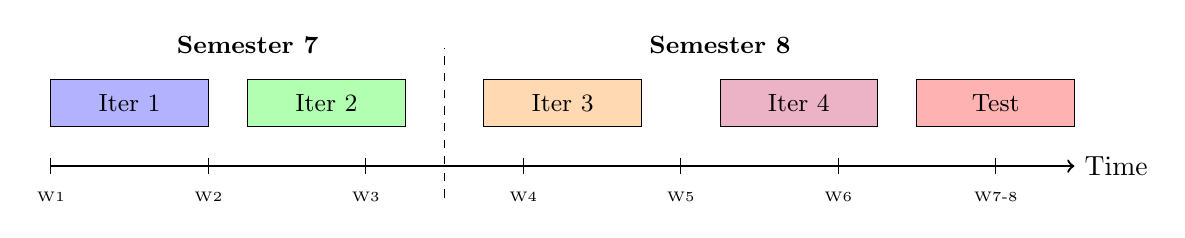
\begin{tikzpicture}[
    phase/.style={rectangle, draw, minimum width=2cm, minimum height=0.6cm, text centered, font=\small},
    milestone/.style={diamond, draw, fill=yellow!50, minimum size=0.4cm}
]

\draw[thick, ->] (0, 0) -- (13, 0) node[right] {Time};

\foreach \x in {0, 2, 4, 6, 8, 10, 12} {
    \draw (\x, -0.1) -- (\x, 0.1);
}
\node[below, font=\tiny] at (0, -0.2) {W1};
\node[below, font=\tiny] at (2, -0.2) {W2};
\node[below, font=\tiny] at (4, -0.2) {W3};
\node[below, font=\tiny] at (6, -0.2) {W4};
\node[below, font=\tiny] at (8, -0.2) {W5};
\node[below, font=\tiny] at (10, -0.2) {W6};
\node[below, font=\tiny] at (12, -0.2) {W7-8};

\node[phase, fill=blue!30] at (1, 0.8) {Iter 1};
\node[phase, fill=green!30] at (3.5, 0.8) {Iter 2};
\node[phase, fill=orange!30] at (6.5, 0.8) {Iter 3};
\node[phase, fill=purple!30] at (9.5, 0.8) {Iter 4};
\node[phase, fill=red!30] at (12, 0.8) {Test};

\draw[dashed] (5, -0.4) -- (5, 1.5);
\node[above, font=\small] at (2.5, 1.3) {\textbf{Semester 7}};
\node[above, font=\small] at (8.5, 1.3) {\textbf{Semester 8}};

\end{tikzpicture}
\captionof{figure}{Development Timeline}
\label{fig:timeline}
\end{minipage}
\vspace{0.5cm}

\subsection{Risk Management}

\noindent
\begin{minipage}{\textwidth}
\centering
\captionof{table}{Project Risk Assessment}
\label{tab:risks}
\small
\begin{tabular}{|p{2.5cm}|c|c|p{5cm}|}
\hline
\textbf{Risk} & \textbf{Prob.} & \textbf{Impact} & \textbf{Mitigation} \\
\hline
AI API rate limiting & High & Medium & Request queuing; multi-provider fallback \\
\hline
Character inconsistency & Medium & High & Reference image injection; prompt optimization \\
\hline
Third-party API changes & Low & High & Abstract provider interface; version pinning \\
\hline
Performance issues & Medium & Medium & Caching; CDN usage; lazy loading \\
\hline
Security vulnerabilities & Low & High & Regular audits; dependency updates \\
\hline
\end{tabular}
\end{minipage}
\vspace{0.5cm}

\section{Summary}

This chapter presented the comprehensive system requirements, architectural design, and development plan for Pixelar. The requirements specification covers functional requirements across user management, generation, project management, and export capabilities, along with non-functional requirements for performance, reliability, security, and usability.

The system architecture follows a modern three-tier design with clear separation between the Next.js frontend, Express.js backend, and Firebase/Vercel data layer. The development plan organizes work into four two-week iterations, with Iterations 1 and 2 completed within Semester 7 establishing core infrastructure and AI generation capabilities.